% Copyright (c) 2010 Jérémie DECOCK (http://www.jdhp.org)

\documentclass{beamer}

\usepackage[utf8]{inputenc}
\usepackage[frenchb]{babel}

\usepackage{subfigure}

\newcommand{\vs}[1]{\boldsymbol{#1}} % vector symbol (\boldsymbol, \textbf or \vec)
\newcommand{\ms}[1]{\boldsymbol{#1}} % matrix symbol (\boldsymbol, \textbf)

\title{Présentation de l'article \emph{An efficient boosting algorithm for combining preferences} \\ 
       (Y.~Freund et al., 1998)}

\author[Rousseau, Decock]{François~\bsc{Rousseau} \and Jérémie~\bsc{Decock}}
\institute{UPMC}
\date{13 octobre 2010}


\AtBeginSection[] {
    \begin{frame}
    \begin{center}
        {\LARGE \insertsectionhead}
    \end{center}
    \end{frame}
}

\begin{document}

%%%%%%%%%%%%%%%%%%%%%%%%%%%%%%%%%%%%%%%

\begin{frame}
    \titlepage
\end{frame}

%%%%%%%%%%%%%%%%%%%%%%%%%%%%%%%%%%%%%%%

\begin{frame}{Plan}
    \tableofcontents
\end{frame}

%%%%%%%%%%%%%%%%%%%%%%%%%%%%%%%%%%%%%%%

\section{Le boosting}

\begin{frame}{Le boosting}
    Face à un problème de classification complexe, il est difficile de
    construire un classifieur 
    \begin{itemize}
        \item efficace
        \item qui généralise bien
    \end{itemize}
    ~\\
    En revanche, il est plus facile de construire un classifieur
    \og{}faible\fg{}
    \begin{itemize}
        \item classant un peu mieux que le hasard
        \item sur un sous ensemble des données
    \end{itemize}
    ~\\
    \begin{block}{Boosting}
        On peut résoudre un problème complexe en combinant intelligement
        plusieurs classifieurs faibles
    \end{block}
\end{frame}

\begin{frame}{Exemple}
    \begin{figure}
        \centering
        \pause \subfigure{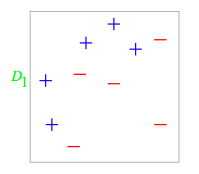
\includegraphics[height=.20\textheight]{fig/0}}~~~
        \pause \subfigure{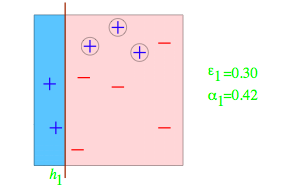
\includegraphics[height=.20\textheight]{fig/1}}
        ~\\
        \pause \subfigure{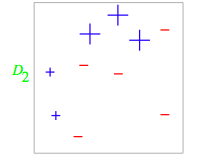
\includegraphics[height=.20\textheight]{fig/2}}~~~
        \pause \subfigure{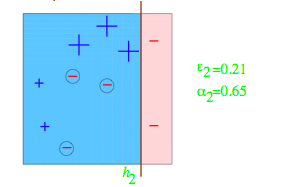
\includegraphics[height=.20\textheight]{fig/3}}
        ~\\
        \pause \subfigure{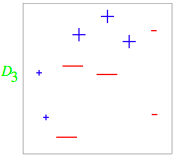
\includegraphics[height=.20\textheight]{fig/4}}~~~
        \pause \subfigure{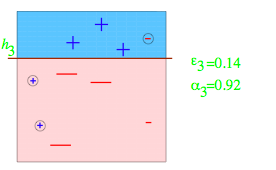
\includegraphics[height=.20\textheight]{fig/5}}
    \end{figure}    
\end{frame}

\begin{frame}{Exemple}
    \begin{figure}
        \centering
        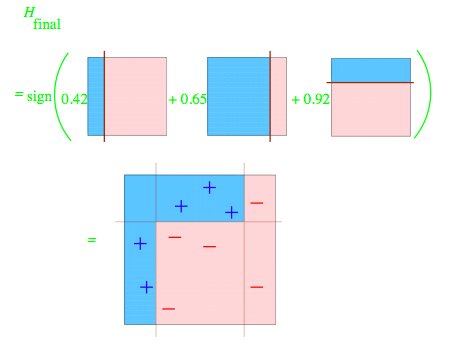
\includegraphics[width=0.5\linewidth]{fig/6}
    \end{figure}    
\end{frame}

\begin{frame}{Historique}
    Historique
    \begin{itemize}
        \item $[$Kearns and Valiant 88$]$~: \emph{does weak learnability
              imply strong learnability~?}
        \item $[$Schapire 90$]$~: premier algorithme prouvé \emph{The strength
              of weak learnability} (boosting par sous ensembles)
        \item $[$Freund and Schapire 95$]$~: Adaboost (l'algorithme de
              référence)
        \item $[$Freund and Schapire 98$]$~: Rankboost
    \end{itemize}
\end{frame}

\begin{frame}{Adaboost}
    \begin{block}{Ensemble d'apprentissage étiqueté}
        $\mathcal{S} = \{ (\vs{x}_{1},y_{1}),\ldots,(\vs{x}_{m},y_{m}) \}$,
        $\vs{x}_{i} \in \mathcal{X}$, $y_{i} \in \{+1, -1\}$, $i = 1, m$
    \end{block}
    \begin{block}{Initialisation la distribution des exemples}
        $D_1(i) = \frac{1}{m}, i=1,\ldots,m$
    \end{block}
    \begin{block}{Déroulement}
        Pour $t = 1,\ldots,T$
        \begin{itemize}
            \item tirer un échantillon d'apprentissage $\mathcal{S}_t$ dans $\mathcal{S}$ selon $D_t$
            \item trouver une \emph{hypothèse faible} $h_{t} : \mathcal{X} \to \{+1, -1\} /
                  h_t = \underset{\epsilon_t}{argmin} $
            \item calculer le poids $\alpha_{t}$ de $h_t$ :
                  typiquement $\alpha_{t}=\frac{1}{2}\textrm{ln}\frac{1-\epsilon_{t}}{\epsilon_{t}}$ 
            \item $D_{t+1}(i) = \frac{ D_{t}(i) \, e^{- \alpha_{t} y_i h_{t}(\vs{x}_{i})} }{ Z_{t} }$, 
                  $Z_{t}$ un facteur de normalisation
        \end{itemize}
    \end{block}
    \begin{block}{Hypothèse finale}
        $H(\vs{x}) = sign(\sum_{t=1}^{T} \alpha_{t} h_{t}(\vs{x}))$
    \end{block}
\end{frame}

%%%%%%%%%%%%%%%%%%%%%%%%%%%%%%%%%%%%%%%

\section{Rankboost}

\begin{frame}{Rankboost}
    On ne fait plus de la classification mais du \emph{ranking}
    \begin{itemize}
        \item ensemble d’instances $\mathcal{X} = \{x_0, \dots, x_m\}$
        \item ensemble de classements $\mathcal{F} = \{f_0, \dots, f_n \}$ \\
              $f_i(x_0) > f_i(x_1) \Leftrightarrow$ \og{} $i$ préfère $x_0$ à $x_1$ \fg{}
        \item distribution des exemples $D(x_i, x_j) = c . max(0, \phi(x_i, x_j))$ \\
              avec $\phi : \mathcal{X}^2 \to \mathbf{R}$ une relation de préférence
        \item $h(x) = 
              \left\{
              \begin{tabular}{lcl}
                    1         & si & $f_i(x) > \theta$ \\
                    0         & si & $f_i(x) \leq \theta$ \\
                    $q_{def}$ & si & $f_i(x) = \phi$
              \end{tabular}
              \right.
              $ \\
              avec $\theta \in \mathbf{R}$ et $q_{def} \in \{0, 1\}$
    \end{itemize}
\end{frame}

\begin{frame}{Rankboost}
    \begin{block}{Initialisation la distribution des exemples}
        $D_1(x_i, x_j) = c . max \{ 0, \phi(xi, xj) \}$
    \end{block}
    \begin{block}{Déroulement}
        Pour $t = 1,\ldots,T$
        \begin{itemize}
            \item \emph{weak hypothesis} $h_t : \mathcal{X} \to \mathbf{R},
                  h_t = \underset{r_t}{argmax},
                  h_t \in \mathcal{H},$ \\
                  $r_t = \underset{x_i, x_j}{\sum} D_t(x_i, x_j) (h_t(x_j) - h_t(x_i))$ 
            \item \emph{poids du classifieur} : $\alpha_t \in \mathbf{R},
                  \alpha_{t}=\frac{1}{2}\textrm{ln}\frac{1 + r_t}{1 - r_t}$
            \item $D_{t+1}(x_i, x_j) = \frac{ D_t(x_i, x_j) \, e^{ \alpha_{t} (h_t(x_i) - h_t(x_j))} }{ Z_{t} }$
        \end{itemize}
    \end{block}
    \begin{block}{Hypothèse finale}
        $H(x) = \sum_{t=1}^{T} \alpha_{t}h_{t}(x)$
    \end{block}
\end{frame} 

%%%%%%%%%%%%%%%%%%%%%%%%%%%%%%%%%%%%%%%

\section{Résultats}

\begin{frame}{Résultats}
    Données
    \begin{itemize}
        \item recommandation de films (sources~:
              \emph{Digital Equipment Corporation})
        \item 61 625 utilisateurs
        \item 1628 films
        \item 2 811 983 classements
    \end{itemize}
\end{frame}

\begin{frame}{Résultats}
    Méthodes comparées
    \begin{itemize}
        \item régression
        \item $K$ plus proche voisin
    \end{itemize}
    ~\\
    Critères de performance
    \begin{itemize}
        \item \emph{disagreement}
        \item \emph{predicted-rank-of top}
        \item \emph{coverage}
        \item \emph{rank-of-predicted-top}
    \end{itemize}
    ~\\
    \begin{block}{Résultats}
    Rankboost $>$ KNN $>$ Regression
    \end{block}
\end{frame}

%%%%%%%%%%%%%%%%%%%%%%%%%%%%%%%%%%%%%%%

\section*{Conclusion}

\begin{frame}{Conclusion}
    Conclusion
    \begin{itemize}
        \item résultats probants sur les exemples de ranking
        \item le boosting permet d'améliorer sensiblement les performances
              des lors que l'hypothèse faible est bien choisie
    \end{itemize}
    ~\\
    Critiques
    \begin{itemize}
        \item comparaison avec des versions très simplifiées des algorithmes
              (surtout pour KNN)
        \item valeurs non mentionnées et à priori arbitraires pour \emph{truly
              top-rated instances}
        \item sensibilité au bruit/valeur aberrante ($<$ exponentielle)
    \end{itemize}
\end{frame}

\end{document}
